%%%%%%%%%%%%%%%%%%%%%%%%%%%%%%%%%%%%%%%%%
% Masters/Doctoral Thesis 
% LaTeX Template
% Version 1.43 (17/5/14)
%
% This template has been downloaded from:
% http://www.LaTeXTemplates.com
%
% Original authors:
% Steven Gunn 
% http://users.ecs.soton.ac.uk/srg/softwaretools/document/templates/
% and
% Sunil Patel
% http://www.sunilpatel.co.uk/thesis-template/
%
% License:
% CC BY-NC-SA 3.0 (http://creativecommons.org/licenses/by-nc-sa/3.0/)
%
% Note:
% Make sure to edit document variables in the Thesis.cls file
%
%%%%%%%%%%%%%%%%%%%%%%%%%%%%%%%%%%%%%%%%%

%----------------------------------------------------------------------------------------
%	PACKAGES AND OTHER DOCUMENT CONFIGURATIONS
%----------------------------------------------------------------------------------------

\documentclass[11pt, oneside]{Thesis} % The default font size and one-sided printing (no margin offsets)

\graphicspath{{Pictures/}} % Specifies the directory where pictures are stored
\usepackage{glossaries}

\usepackage[square, numbers, comma, sort&compress]{natbib} % Use the natbib reference package - read up on this to edit the reference style; if you want text (e.g. Smith et al., 2012) for the in-text references (instead of numbers), remove 'numbers' 
\hypersetup{urlcolor=blue, colorlinks=true} % Colors hyperlinks in blue - change to black if annoying
\title{\ttitle} % Defines the thesis title - don't touch this

%Acronyms
\newacronym{MRS}{MRS}{Movie Recommendation System}
\newacronym{IMDB}{IMDB}{Internet Movie Data Base}
\newacronym{MVP}{MVP}{Minimum Viable Product}
\makeglossaries

\begin{document}

\frontmatter % Use roman page numbering style (i, ii, iii, iv...) for the pre-content pages

\setstretch{0.3} % Line spacing of 1.3

% Define the page headers using the FancyHdr package and set up for one-sided printing
\fancyhead{} % Clears all page headers and footers
\rhead{\thepage} % Sets the right side header to show the page number
\lhead{} % Clears the left side page header

\pagestyle{fancy} % Finally, use the "fancy" page style to implement the FancyHdr headers

\newcommand{\HRule}{\rule{\linewidth}{0.5mm}} % New command to make the lines in the title page

% PDF meta-data
\hypersetup{pdftitle={\ttitle}}
\hypersetup{pdfsubject=\subjectname}
\hypersetup{pdfauthor=\authornames}
\hypersetup{pdfkeywords=\keywordnames}

%----------------------------------------------------------------------------------------
%	TITLE PAGE
%----------------------------------------------------------------------------------------

\begin{titlepage}
\begin{center}

\centering

\includegraphics[scale=0.25]{Pictures/Logo.pdf} % University/department logo - uncomment to place it

\textsc{\LARGE \univname}\\[1cm] % University name
%\textsc{\Large Minor Thesis}\\[0.5cm] % Thesis type

\HRule \\[0.4cm] % Horizontal line
{\huge \bfseries \ttitle}\\[0.4cm] % Thesis title
\HRule \\[1.5cm] % Horizontal line
 
\begin{minipage}{0.4\textwidth}
\begin{flushleft} \large
\emph{Author:}
\href{}{Nayan Singh Ravindra} % Author name - remove the \href bracket to remove the link
\end{flushleft}
\end{minipage}
\begin{minipage}{0.4\textwidth}
\begin{flushright} \large 
\emph{Examiner:}
\href{}{Dr. Terrence E. Brown}
\end{flushright}
\begin{flushright}
\emph{Supervisor:}
\href{}{Mr. Andres R. Portilla} % Supervisor name - remove the \href bracket to remove the link 
\end{flushright}

\end{minipage}\\[3cm]
 
\large \textit{A thesis submitted in fulfilment of the requirements\\ for the degree of \degreename}\\[0.3cm] % University requirement text
\textit{in}\\[0.4cm]
\groupname
%\\\deptname\\[2cm] % Research group name and department name
 
{\large \today}\\[1mm] % Date
%
\includegraphics{Logo} % University/department logo - uncomment to place it
\end{center}
\end{titlepage}

%----------------------------------------------------------------------------------------
%	DECLARATION PAGE
%	Your institution may give you a different text to place here
%----------------------------------------------------------------------------------------

%\Declaration{
%
%\addtocontents{toc}{\vspace{1em}} % Add a gap in the Contents, for aesthetics
%
%I, \authornames, declare that this thesis titled, '\ttitle' and the work presented in it are my own. I confirm that:
%
%\begin{itemize} 
%\item[\tiny{$\blacksquare$}] This work was done wholly or mainly while in candidature for a research degree at this University.
%\item[\tiny{$\blacksquare$}] Where any part of this thesis has previously been submitted for a degree or any other qualification at this University or any other institution, this has been clearly stated.
%\item[\tiny{$\blacksquare$}] Where I have consulted the published work of others, this is always clearly attributed.
%\item[\tiny{$\blacksquare$}] Where I have quoted from the work of others, the source is always given. With the exception of such quotations, this thesis is entirely my own work.
%\item[\tiny{$\blacksquare$}] I have acknowledged all main sources of help.
%\item[\tiny{$\blacksquare$}] Where the thesis is based on work done by myself jointly with others, I have made clear exactly what was done by others and what I have contributed myself.\\
%\end{itemize}
% 
%Signed:\\
%\rule[1em]{25em}{0.5pt} % This prints a line for the signature
% 
%Date:\\
%\rule[1em]{25em}{0.5pt} % This prints a line to write the date
%}
%
%\clearpage % Start a new page

%----------------------------------------------------------------------------------------
%	QUOTATION PAGE
%----------------------------------------------------------------------------------------

%\pagestyle{empty} % No headers or footers for the following pages
%
%\null\vfill % Add some space to move the quote down the page a bit
%
%\textit{``Thanks to my solid academic training, today I can write hundreds of words on virtually any topic without possessing a shred of information, which is how I got a good job in journalism."}
%
%\begin{flushright}
%Dave Barry
%\end{flushright}
%
%\vfill\vfill\vfill\vfill\vfill\vfill\null % Add some space at the bottom to position the quote just right
%
%\clearpage % Start a new page

%----------------------------------------------------------------------------------------
%	ABSTRACT PAGE
%----------------------------------------------------------------------------------------

\addtotoc{Abstract} % Add the "Abstract" page entry to the Contents

\abstract{\addtocontents{toc}{\vspace{1em}} % Add a gap in the Contents, for aesthetics
Competitor analysis is a key step during innovation process to obtain a reasonable amount of information regarding major players in current industry. It helps a firm to channelize all their efforts in outranking its competitors by developing innovative competitive strategies for the product. This work studies the aspect of comparing features provided by competitor movie recommendation engines that would help in understanding the influence of technological differentiation of a product in achieving sustainable competitive advantage. It also provides suggestions for facing the challenge of achieving technological differentiation in the context of movie recommendation engines. 

 With the help of web based research valuable information is collected about major competitors. A comparison study is carried out to provide a bird's eye view of popular features and thereby accelerating the decision process about inclusion of features in later stages of product development, especially during ideation phase of the process. The study confirms that the there is a positive influence of technical differentiation of product and its success in the area of movie recommendation websites. It also identifies few of the technical and business oriented solutions to achieve competitive edge. 
}

\clearpage % Start a new page

\keywordnames
%----------------------------------------------------------------------------------------
%	ACKNOWLEDGEMENTS
%----------------------------------------------------------------------------------------

%\setstretch{1.3} % Reset the line-spacing to 1.3 for body text (if it has changed)
%
%\acknowledgements{\addtocontents{toc}{\vspace{1em}} % Add a gap in the Contents, for aesthetics
%
%The acknowledgements and the people to thank go here, don't forget to include your project advisor\ldots
%}
%\clearpage % Start a new page

%----------------------------------------------------------------------------------------
%	LIST OF CONTENTS/FIGURES/TABLES PAGES
%----------------------------------------------------------------------------------------

\pagestyle{fancy} % The page style headers have been "empty" all this time, now use the "fancy" headers as defined before to bring them back

\lhead{\emph{Contents}} % Set the left side page header to "Contents"
\tableofcontents % Write out the Table of Contents

\lhead{\emph{List of Figures}} % Set the left side page header to "List of Figures"
\listoffigures % Write out the List of Figures

%\lhead{\emph{List of Tables}} % Set the left side page header to "List of Tables"
%\listoftables % Write out the List of Tables
\printglossary[type=\acronymtype,title=Acronyms]

%----------------------------------------------------------------------------------------
%	ABBREVIATIONS
%----------------------------------------------------------------------------------------

%\clearpage % Start a new page
%
%\setstretch{1.5} % Set the line spacing to 1.5, this makes the following tables easier to read
%
%\lhead{\emph{Abbreviations}} % Set the left side page header to "Abbreviations"
%\listofsymbols{ll} % Include a list of Abbreviations (a table of two columns)
%{
%\textbf{LAH} & \textbf{L}ist \textbf{A}bbreviations \textbf{H}ere \\
%%\textbf{Acronym} & \textbf{W}hat (it) \textbf{S}tands \textbf{F}or \\
%}

%----------------------------------------------------------------------------------------
%	PHYSICAL CONSTANTS/OTHER DEFINITIONS
%----------------------------------------------------------------------------------------

%\clearpage % Start a new page
%
%\lhead{\emph{Physical Constants}} % Set the left side page header to "Physical Constants"
%
%\listofconstants{lrcl} % Include a list of Physical Constants (a four column table)
%{
%Speed of Light & $c$ & $=$ & $2.997\ 924\ 58\times10^{8}\ \mbox{ms}^{-\mbox{s}}$ (exact)\\
%% Constant Name & Symbol & = & Constant Value (with units) \\
%}
%
%----------------------------------------------------------------------------------------
%	SYMBOLS
%----------------------------------------------------------------------------------------

%\clearpage % Start a new page
%
%\lhead{\emph{Symbols}} % Set the left side page header to "Symbols"
%
%\listofnomenclature{lll} % Include a list of Symbols (a three column table)
%{
%$a$ & distance & m \\
%$P$ & power & W (Js$^{-1}$) \\
%% Symbol & Name & Unit \\
%
%& & \\ % Gap to separate the Roman symbols from the Greek
%
%$\omega$ & angular frequency & rads$^{-1}$ \\
%% Symbol & Name & Unit \\
%}

%----------------------------------------------------------------------------------------
%	DEDICATION
%----------------------------------------------------------------------------------------
%
%\setstretch{1.3} % Return the line spacing back to 1.3
%
%\pagestyle{empty} % Page style needs to be empty for this page
%
%\dedicatory{For/Dedicated to/To my\ldots} % Dedication text
%
%\addtocontents{toc}{\vspace{2em}} % Add a gap in the Contents, for aesthetics
%
%----------------------------------------------------------------------------------------
%	THESIS CONTENT - CHAPTERS
%----------------------------------------------------------------------------------------

\mainmatter % Begin numeric (1,2,3...) page numbering

\pagestyle{fancy} % Return the page headers back to the "fancy" style

% Include the chapters of the thesis as separate files from the Chapters folder
% Uncomment the lines as you write the chapters

% Chapter 1

\chapter{Introduction} % Main chapter title

\label{Chapter1} % For referencing the chapter elsewhere, use \ref{Chapter1} 

\lhead{Chapter 1. \emph{Introduction}} % This is for the header on each page - perhaps a shortened title

\setstretch{1}
%----------------------------------------------------------------------------------------
\section{About recommendation engine industry:}
 
 Recommendation engines aim at providing personalized suggestions to its users based on their behavior and taste, thereby reducing time taken to search a particular product or information in the web. Most of the recommendation engines are website based, few noticeable industry participants are Amazon, \acrshort{IMDB}, Flip-kart, eBay, Google, Linked-in, Facebook and Netflix. Main purpose of recommender websites is to cater for need of the customer by providing suggestive list of web pages as in case of Google, or to suggest relevant jobs as in the case of Linked-in or it could be suggesting next product to buy for users as in the case of on-line retail stores. Facebook uses it to filter posts from friends and for suggesting new friends, it is also used to predict movies matching to user's preference and tastes as in the case of Netflix. Recommendation engines have gained popularity with the advent of big data, a lot of startups have been created based on the idea of providing recommendations to its users. It helps users by filtering humongous amount of irrelevant data and by providing most relevant suggestions. Based on type of data used by recommendation engines, it is capable of either suggesting movies, restaurants, products or books to its users \citep{Recom0}. 

 Our main concern is about movie recommendation engine industry, which is built on data related to movies provided by movie industry from all over the world. Considerable amount of movies are added into movie database from movie producers each year, it is to be noted that there are more than hundred million movie titles in \acrshort{IMDB}, a largest on-line movie database \citep{IMDb2}. It also contains information about movie related data such as character, actor, popularity based information. Given this amount of data involved, movie data can be safely classified as big data. Currently there are about 15-20 companies in the area of on-line movie recommendations by either providing suggestions based on movie content, based on collected data from users or using both to predict and provide better suggestions. The top five companies in this domain are listed in decreasing order of popularity, they are \acrshort{IMDB}, Fandango, Rotten tomatoes, Flixster, What to rent ?. 

 A on-line movie on demand company, Netflix utilizes the power of movie recommendations to increase its customer engagement and it has also reported that due to recommendations, the subscriber growth is in the range of 10 to 30 percent \citep{Here1}. Movie recommendation engines are quite popular among movie enthusiasts, live example is popularity of \acrshort{IMDB} website with an average monthly traffic of 15 million users in USA alone \citep{Imdb8}, making it one of the top hundred most visited websites in the world as shown in \citep{Alexa5}. The example provided above establishes the fact that there is an imminent demand for movie recommendation engines and also in future due to monotonic increase in addition of new movies into the database. 

 It is clear from the above context that there is future for companies building movie recommendation engine. Competition is fierce due to involvement of major players in recommendation systems, namely \acrshort{IMDB}. There is a need for innovation in movie data analytics area and also in the domain of accurately predicting behavior of users to improve the state of movie recommendations provided. Availability of open source movie data reduces barriers for a new company to enter into recommender market. Typically, a company with a most innovative recommender algorithm involving in-depth movie content analysis, social data analytics, excellent user friendly framework for content discovery and moderate web infrastructure would be able to reach out to customers from all around the world with the help of a website. Generally, in the area of movie recommendation engines revenue models are based on advertisements in web space, royalties for publishing movie information, movie tickets sales, sales of collected customer data to other companies and end user subscription based revenue model.       

\section{About the company and its product:}
 Internship is carried out in a five year old startup company named Vion Labs, Stockholm. It is a digital media technology startup which focuses on providing a state of the art, innovative and appealing product for movie enthusiasts in the form of movie recommendation engine. A recent study by eMarketer in USA expects that an US adults to spend around 5 hours 46 minutes of their time per day in getting involved in digital media \citep{Mobil1}. As per movie on demand provider NetFlix, it has been observed that a average subscriber spends approximately 1 hour and 44 minutes streaming the video content \citep{HowM2}. From these studies it is clear that an average person spends most of his leisure time involving activities like watching movies, television and playing games in the digital world. Hence our startup has been focusing on digital media market to target a large number of customers in this segment. 

The method used for describing product or a service provided by a company is based on these following areas:
 
  \subsection{Features} % (fold)
  \label{sub:features}
  % subsection features (end) 
  The stand out and most attractive attributes that a company can offer in a product is a feature. The latest product of Vion labs is named as  ``Vionel'', which is a website with a personalized movie discovery platform. It has an appealing user friendly front end containing information about latest movies. It also has information about content providers, from where the users can get access to the video content. One of the attractive feature of Vionel is that it provides a social media type of platform to share personal views, likes and dislikes about a movie in the form of comments.
  
  The recommendation engine assigns a rating percentage score based on popularity of a movie, which helps user to chose movies with highest ratings. The front end of website provides user with the options to list movies based on different genres, keywords and characters involved. The feature of searching movies based on the tags for example,``adventure, action,comedy etc'' is also a part of Vionel's front-end.

  Vionel provides its users with a lot of different dimensions for critically analyzing movies. Future features to be included in website include relationship graphs among characters in the movies. Advertisement free web interface is one of the stand out feature of Vionel product, which creates a non-intrusive environment for the users to browse through movies. On the other hand it provides an excellent platform for the partner companies and other movie franchises to publish their movies in website.      
      
  \subsection{Advantages} % (fold)
  \label{sub:Advantages}
  % subsection subsection_name (end){Advantages} 
  Vionel is capable of providing its users with an state of the art movie content discovery platform unlike its competitors. The main advantage of Vionel is that it provides an user friendly social media platform for discussing and sharing one's view about the movies and the characters in the movies.

  The feature of bookmarking one's choice of movies and storing it in one's profile is a new feature in web movie database websites and Vionel has this feature. Vionel provides movie franchise owners to advertise their movies and trailer videos related to the movie. It also provides movie creators with social advertisement platform to collect opinions about movies from the viewers.      	   
   
  \subsection{Returns for the customer}
  \label{sub:Returns for the customer}

  Vionel provides its customers with a free website to enrich their movie selection experience. It provides users with a personalized movie discovery website with option to bookmark movies and also provides pointers to where the users can access the movie content. It also provides a user friendly social environment to discuss one's views about the movies. The website provides a one stop solution for all the movie enthusiasts to ponder upon latest content in the entertainment world and stumble upon movie to watch in lesser time than searching in web. It provides the movie creators and its advertisement agencies to showcase trailers of the movies. It enables movie franchises to collect valuable opinions and general public comments about the movies. Finally, the new and innovative features that are planned to be a part of Vionel product are from the internship work of automatic brand logo detection in movies to generate tag or category of movies namely ``Movies with product placement''. Along with recommendation engine this tag is used to provide better suggestions for the users of Vionel. Thereby assisting the movie recommendation engine to showcase the list of best possible movies based on user's choice and search behavior.      
 
%----------------------------------------------------------------------------------------
\section{Details about major thesis and its relevance}
% Explain about logo detection in movies, product placement in movies, how it can be automated way of creating a separate tag as an input to movie recommendation engines. Currently how rotten tomatoes, \acrshort{IMDB} are creating this tag ? {using user's reviews and comments}. This process can be automated and credibility of the data can be maintained. Block diagram of the movie recommender engine (Write this in essay part of the report ) Which Phase ? Why so ? %
%----------------------------------------------------------------------------------------
 Goal of major thesis and internship is to develop a automatic brand logo detection in input movies. Recognition, identification of brand logos in movies is a arduous and error prone task to be carried out by humans. In order to accelerate the process of detecting logos and also to increase the accuracy of detection in movies a machine learning algorithm combined with computer vision algorithms are used. The process of analyzing more than hundred million movies to detect the presence of brand logos is a time consuming process, hence in the project a cluster of state of the art graphical processing units are used to accelerate the process. After detection of logos, movies are tagged as containing product placement in them. The tags generated for all the movies are collected and used as input to movie recommender system. An instance of the use case is, when a user has liked watching movie with product placements, it is highly likely a user may like another movie with similar tag. Hence in order to increase the reliability of movie recommendation engine, a lot of such features has to be developed. The deliverable of internship will be to automate the process of movie logo detection and generate output in a predefined structure, to be later used by recommender system. Currently brand logo detector is in prototyping phase of software development cycle.

\section{Current phase in innovation process} 
%----------------------------------------------------------------------------------------
 % About the process and current phase of minor thesis 
 Company has developed a \acrshort{MVP} in the form of a movie information publishing and discovery platform. The \acrshort{MVP} has been launched in the market as a website named \href{www.vionel.com}{Vionel}. The baseline release of the product has the feature of allowing users to search for movie information, provide comments about movie content, share and bookmark movies. It lacks recommendation engine that provides user with personalized recommendations based on data collected from behavior of users. Hence current goal of research and development team of the company is to develop a state of the art movie recommender engine, which provides a reliable set of movie recommendations to the end user. 
 \par Since recommendation engine is a new feature going to be added on top of baseline product, there is need to study business aspects like demand from customers, current market scenario and about competitors. Recommendation engine product is currently in ideation phase of innovation process framework. In this phase R\&D team brainstorms about type of recommender system to use, set of innovative features to be included and aspects about increasing accuracy of suggestions. One such feature is part of my internship project involving automatic brand logo detection in movies, which is currently in prototyping phase of its software development cycle. The final output of master thesis project is to produce tag information for movies with product placements, it will be one of the many inputs for final recommender engine product. Likewise, there are other innovative features that could be included as part of the movie recommendation engines, such as creation of tags for movies with a particular type of environment (ex: Indoor, Forest, Urban etc). 
 \par Prior to ideation phase in innovation process, two important steps has to be performed. First one is to investigate needs and demands of the customer in recommender system context. Second step is to investigate about current market situation for product that is intended to be created. These two steps clears out the confusion regarding acceptance of end product by customers. The next step is to understand competition in the field by performing competitor analysis. Subsection \ref{Voice} explains about problems, needs and demand of customer in recommender engine context and it also gives insight about current market scenario in web based recommender systems.

 \subsection{Voice of the customer}
 \label {Voice}
  % Movie recommendations acceptance poll by the customers (a graph may be). Need for recommendations, what problems are faced by the customer currently ? How our solution mitigates it ? Demand discovery. Block diagram of voice of customer, explain each of the blocks. 
  Customer demand always drives success of a product. Discovery, timely identification and capitalization of customer demand about a particular product is essential for development of a company. Value proposition as perceived by customer should be in positive note, also a product or service should be a able to solve a problem faced by the customer. During initial phase of market study, needs, expectations and preferences of movie recommendation engines are studied.
  \par
  In the case of simple movie discovery and information retrieval websites, customers face problem of manually searching movies they want to watch at that instant and it is a time consuming task especially if the number of choices are large in number. This is a problem, since each time a user logs into a movie discovery website, the set of movies displayed will be static with latest movies getting priority of moving up the list. The list presented is identical for all the users, which makes majority of users to leave the service. Hence it is observed that customers need a personalized list of movie suggestions based on their taste, mood, time and day of the week and other user information. It is also noticed that when an average user has no preference about movie to watch, always takes suggestions from a friend before watching a movie. This limits the possibilities of movies suggested by a friend, this demands recommendation engines to be automated and personalized to enrich and surprise users by providing diversified set of movie suggestions when compared to suggestion from a friend.
  \par 
  Direct demands and other implicit information about a product is obtained using a market survey. One such survey conducted in 2010 as in figure \ref{fig: Familiarity of recommendation engines} showed that more than 80 percent of the respondent population either showed interest in recommendation engines or currently using one \citep{Recom8_voc}. This study reveals information about the familiarity of recommendation engines by customers. 
 
  \begin{figure}[htbp]
	\centering
		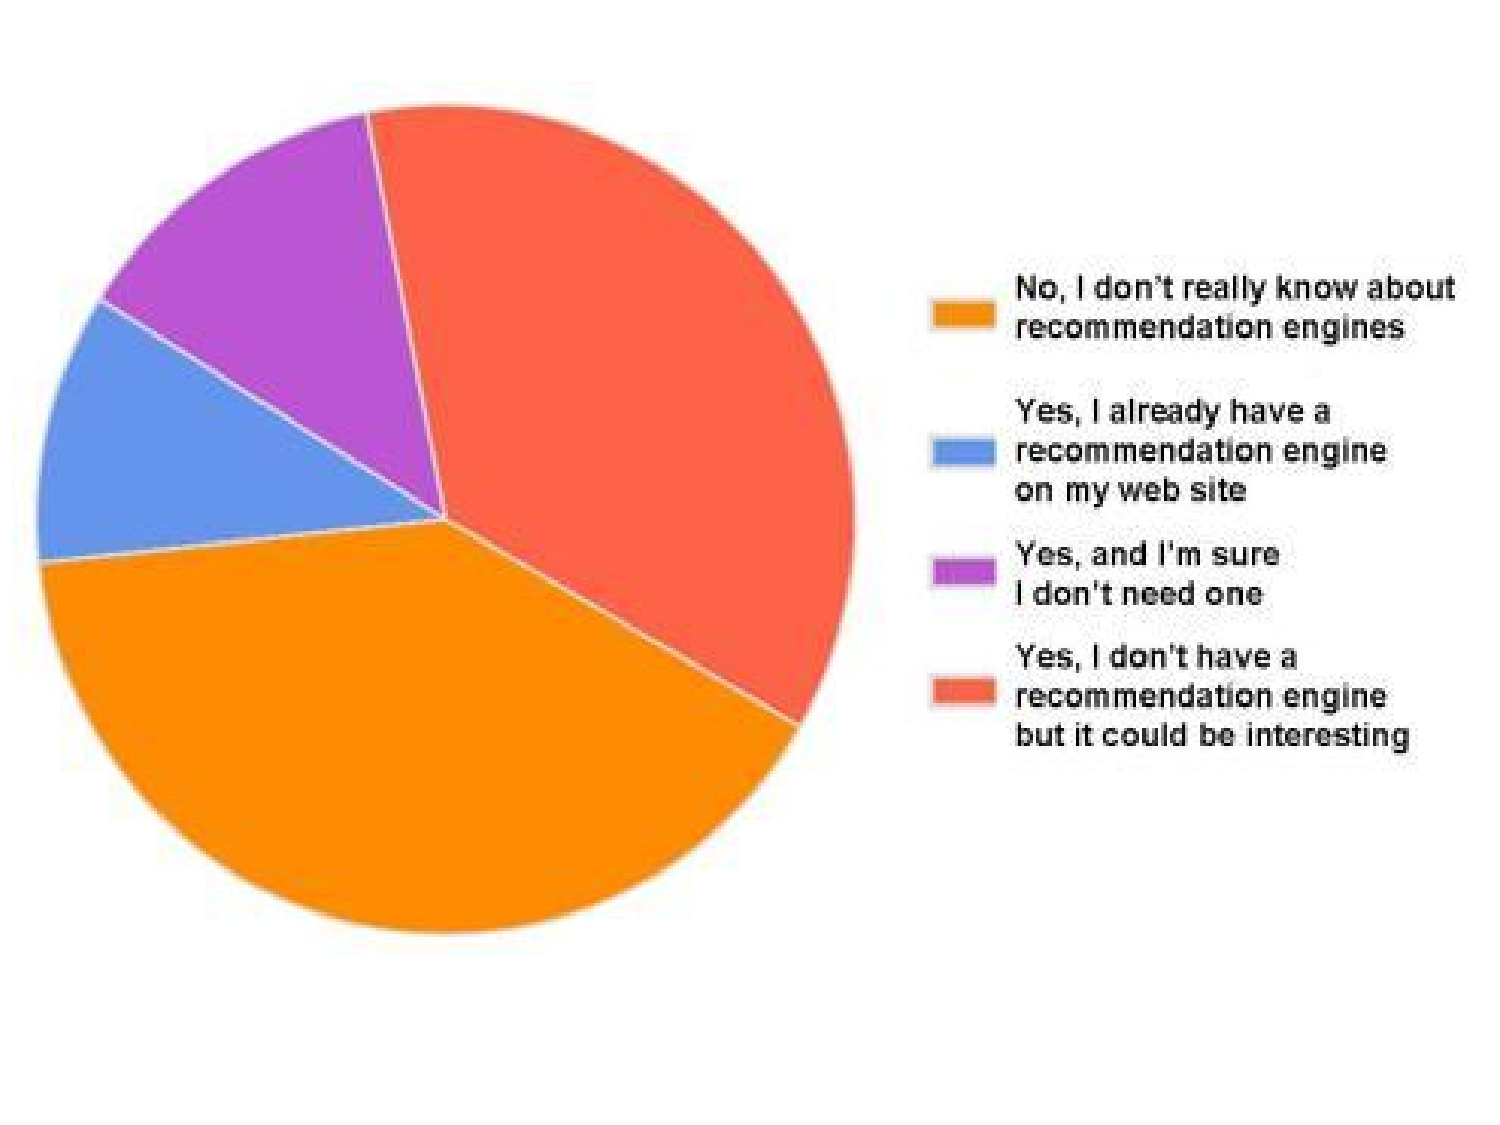
\includegraphics[scale=0.4]{Figures/familiarity_recommendation_engines.pdf}
		%\rule{35em}{0.5pt}
	\caption[Graph: Familiarity of web based recommendation systems]{A survey results on familiarity of recommendation engines \citep{Recom8_voc}.}
	\label{fig: Familiarity of recommendation engines}
  \end{figure} 

  Public relation(PR) team members in Vion Labs have been able to build a good relationship with current users of Vionel using social media and emails. Customer view about the product is obtained from feedback forms in the website. Evenmore personalized review comments about website and its content are obtained by sending out emails for first five hundred privileged users. Complaints, suggestions about movie information are logged and periodically checked to improve the service. The availability of baseline website made the process of understanding customer views about inclusion of recommender system using surveys a easy task, the response gathered is positive about movie recommendations inclusion. Vionel is a free website for users from all over the world, along with that inclusion of state of the movie recommendation enriches movie selection experience of customers. In order to gain even more insights from customers, an interactive video linked with a on-line survey was prepared and published to gather information. In conclusion, there is a positive demand for movie recommendation engine by end users. 

  Marketing team have gathered information about benefits for partner companies and movie franchises, by inclusion of recommendation features on top of baseline product. It has been observed that movie recommendations diversifies the spread of movies chosen by users and thereby increasing the sales of less familiar DVDs and video content from partner websites such as Netflix. This boosts movie content that is not so popular among public, hence movie on demand services can benefit from less familiar movies available in unprofitable part of long tail distribution of movies as discussed in \citep{Profile_online}.

  Even though, initial analysis of customer needs, problems and expectations are accomplished, there is a room to investigate more and understand average customer expectations about movie recommendation engines. The view of recommendations as perceived by the user, will highly influence both technical and business decisions during the development of \acrshort{MRS}. More customer insights about outlook of a recommender system is to be collected using customer interviews, surveys and discussion with movie franchise owners. More data needs to be collected about user's opinion on intrusion levels of privacy for collecting user behavioral data on website such as clicking pattern on displayed movie information, movie posters viewed, searching pattern for movies, comments, bookmarks, likes and dislikes of displayed movies.

  Marketing team in Vionel have collected information from web regarding market share information of recommendation engines. Google page rank of websites provide information about the number of unique views of the website, which is used to calculate market share of various recommendation engines. Sector graph in figure shows the market share information of the websites the data is collected and computed from from \citep{Alexa_imdb}. It is assumed that the company which has least rank has highest market share. It is observed that \acrshort{IMDB} has captured a market share of more than 88 percent. The reason is due to it sheer movie information database and presence of user ratings. There is still room for conducting market survey to understand about competitors in current scenario.      
   
  \begin{figure}[htbp]
	\centering
		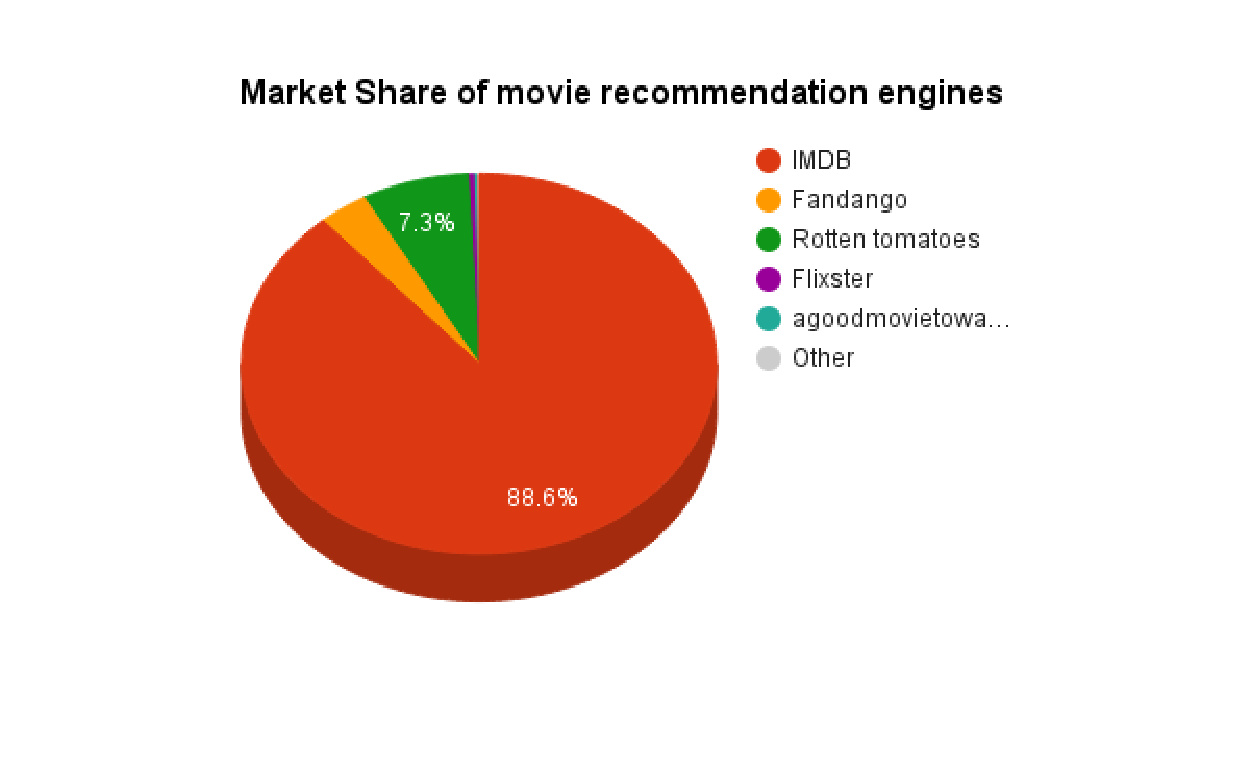
\includegraphics[scale=0.5]{Figures/Market_share.pdf}
		%\rule{35em}{0.5pt}
	\caption[Sector graph: Market share of web based recommendation systems]{Market share of web based movie recommendation engines \citep{Alexa_imdb}.}
	\label{fig: Market share information of web based movie recommendation systems}
  \end{figure} 

% \subsection{Market analysis}
% \label {Market}

 % What is it ? its importance ? its role in driving innovation strategy ? 
 
 % Real market facts and figures, market share, TAM,
 
 % Ideation of the product : Unique features inclusion into baseline product.
 

\section{Framing of business research question in the given context}
%----------------------------------------------------------------------------------------
 % How to achieve competitive edge, comparison of tech, business features, marketing strategies, strategic alliances made by other companies, attaining competitive sustainable advantage---> The process (innovative framework) for quick reference comparison.  
 Baseline version of the product Vionel has been launched in the market, but it lacks movie recommendation engine. There has been a considerable amount of effort spent in understanding needs, problems and expectations of customer regarding movie recommendation engines. The second part of the study involved study of market in context to acceptance of movie recommendation engines. A movie recommendation engines is an ensemble of various features both related to movie content and user behavior. Development and inclusion of each feature for a movie recommendation engines is a project with an aim of analyzing movies and generating movie tags in an innovative way. The reliability, accuracy and popularity of \acrshort{MRS} depends on the features it has and quality of tags it holds. 

 As a step along innovation process framework it is required to understand about competitors in movie recommendation engines, features used and provided to the end users. Comparison with competition helps us to improve the present condition of \acrshort{MRS} by either addition or deletion of features. Knowing about competition much before ideation phase of innovation process, helps R\&D team members to collaborate and come up with quality features to be added on top of baseline version. So there is a benefit of performing detailed analysis about competition to further reduce the development time of \acrshort{MRS}. This helps company to achieve shorter time to market for the product by taking appropriate measures during ideation phase of the product. Hence the research question that will be answered in this minor thesis would be about  

 \textbf{RQ}: \textbf{``How to investigate with a creative approach and compare features provided by movie recommendation engine firms. Also based on this, to develop a consistent understanding of how technological differentiation in technical features of a movie recommender website would attract more number of users to gain sustainable competitive advantage in an innovative way ?''}
% Chapter 1
\chapter{Literature Study} % Main chapter title

\label{Chapter2} % For referencing the chapter elsewhere, use \ref{Chapter1} 

\lhead{Chapter 2. \emph{Literature Study}} % This is for the header on each page - perhaps a shortened title

\setstretch{1}
%----------------------------------------------------------------------------------------

Business research question that will be addressed in this report concerns about detailed competitor analysis in the sector of movie recommendation engines. The task involves identification of competitors, investigation of the features provided by the competitors as compared to Vionel as a step forward in the business innovation process. The following paragraphs explains about background, need for recommendations, general problems of customer and the efforts of movie recommendation engine companies to solve problem of customers. It also explains about features supported by state of the art movie recommendation engines in current market.

\section {Background}

Every person spends a considerable amount of time in leisure activities by getting involved in recreational sports, surfing the web, watching television or other digital entertainment. With the advent of web and digital media technology, there has been an increase in time spent by  individuals on-line. It is also noticed that the trend of socializing through web has increased with the introduction of social media websites. As per a recent study, it has been observed that Americans, who do use computers for leisure spend a considerable amount of time per day watching digital content or playing on-line games and it is approximately of about hundred minutes per day \citep{time_spent_online}. Although the study did not mention about correlation of time spent on-line with variables such as time of the day, day of the week, age, occupation and other demographical information. It is clear that few aspects such as income and occupation plays an important role in influencing on-line presence of an individual. Nowadays, a larger chunk of those hundred minutes is spend in watching movies, television series and other videos available in social video sharing websites such as you-tube, vimeo etcetera.

Before computers took over the world, till the late of twentieth century people had access to media content, especially movies only through television and cinema theaters. Also the number of movies and other media content produced by year was considerably less as compared to current scenario the reason being due to introduction of state of the art technology. As per a recent statistical study by Statista website \citep{number_of_movies_per_year_online} the number of movies released per year has been consistently growing, this creates a favorable environment for businesses related to movies and digital entertainment. Movie franchises that are producing interesting movies for the viewers become the strongest complementer for our product. And also mobile gadgets companies, entertainment product manufacturers are assisting our service in an indirect way by increasing availability, ease of web access in various hand held mobile devices to get people engaged in digital media content for a longer duration of time. The information of time spent by an individual in a website is an actionable and interesting metric for the creators of the website. Naturally, given an average time spent by users, the owner of a website could estimate quality and popularity among the people on-line. Main objective of any website creator is not only to attract more number of unique visitors but also to engage them to spend more time by providing quality content. It also enables users to publish content into the web, on the other hand users have an access to large volumes of information at their convenience. 

\section{Need for movie recommendations}

The problem with availability of more information at one place is that it could create a sense of confusion for the users to decide and chose suitable information from the available content especially if the options are equally good. The scenario in which users face ``what to watch ?'' barricade is a highly common occurrence in the case of on-demand content delivery services, especially in the case of movie on demand services, in which users can chose and watch a movie on-line in their leisure time. If the user has less clue about movie to watch, it can be really time consuming for the user to decide upon and chose a particular movie to watch. Also a lot of user's time can be spent on searching the on-line content to find the appropriate type of movie one likes to watch. When users are presented with more than million choices of movies to watch, as in the case of Netflix, the users have trouble in choosing a best content from the lot \citep{flicking_online}. In this scenario most of the users tend to switch to other websites or decide not to watch movie at that instance, which highly affect popularity of movie on demand service. In order to develop a better rapport with the users the companies have come up with an solution to assist its users in choosing movies to watch by providing suggestive list of movies. The software that provides suggestions is termed as a recommendation engine and in this particular case a movie recommendation engine. It solves the problem of user's confusion of choosing and deciding the movie content to watch.

\section{State of the art movie recommendation engine}
\label{State of the art movie recommendation engine}
An ideal movie recommendation engine would present user with a personalized list of accurately predicted movies based on movie content, user's mood, taste and other behavioral aspects. It should be able to replace search engines for a movie recommender website, a user should be able to view the list of suggestive movies instead of manually searching for the movies one likes. The list of movies suggested by the recommender system should be accepted by the user at that instance, failure to do so might disappoint user and eventually one might loose trust over the generated results. A recent study about \acrshort{MRS} of Netflix shows that the predicted results include both blockbuster movies and movies that are less popular, this mix of suggestions motivates user to consume content from both categories \citep{Longtail_online}. Hence in a competitive market, there is a need for continuous innovation in recommender systems for predicting accurately movies needed by the customer at a given point in time. The accuracy and hence popularity of a movie recommendation system completely depends on the criteria used for generating predictive results. The predicted results can be solely based on features of a movie, its actors, directors, plot or it could be based on similarity between movies watched by user earlier and the current database of movies. The prediction list of movies should include movies that surprise the user, an example would be a list containing all action films except few of them belonging to other genre category which have similar directors, actors, speed of the movie, movie color tone and plot. It is also essential for an recommender engine to explain the reason for inclusion of such movies in the predicted results to convince users about its relevance in the list and there should be provision for the users to validate the generated results.  

A popular recommender engine should be able to generate diversified, relevant, personalized, customized, intriguing and dynamic results for each user. Nowadays, with the growth of digital social media a user can get information about latest movies, which is not the case for old movies that not popular and also movies that belong to a different geographic location. It is a good to have feature for recommender engine to be able to learn individual user's taste and to include these results in the recommendations. In a broader sense, recommender systems can be categorized into collaborative filter based, content based and hybrid recommender system \citep{Article_1}. It is observed that users generally choose movies with a similar kind of qualities, the system that learns about the user preferences over a period of time in a non intrusive way and uses the collected data as input to generate suggestions in future for the users is collaborative filtering based \acrshort{MRS}. Whereas content based \acrshort{MRS} predicts a list of movies to the user based on the similarity between preselected set of movies obtained from the user and database of movies. The last category of \acrshort{MRS} combines the idea of both content and collaborative based systems to refine the results and generate highly accurate results for the users. There is a shortcoming in case of recommendation engines referred to as cold start problem, which means that algorithm has very less information about a user to provide recommendations, this is the case for all new users. Hence availability of user data plays an important role in determining quality of recommendations.

In order to perform competitor analysis there is a need to understand features of a ideal \acrshort{MRS} in order to achieve comparatively better results from the competitors. Also a study of both technical and business strategies used by the competitors is required to learn from their mistakes and better our service.           

\section{About our competitors}

 After understanding needs of customer and market scenario for a product, next step is to know about competition. Competitors are the companies in similar domain or a similar product, a service offering owned by a company that poses threat to promotion of our product and competes to be popular among common customer segment. In essence, any entity that competes against our company by fighting for market share in the niche segment by providing better value to the customer for lower price or investment. The process of discovering competitors involves a lot of research using new papers, popular magazines in the domain, press releases, business articles and data available on-line. Filtering and shortlisting the competitors is crucial before performing a detailed competitor analysis by avoiding traps of considering a company with no relevance as a competitor, on the other hand missing out a tough competitor could prove to be fatal for company's future. Competitor analysis provides decision makers with an valuable data about current scenario, which assists them to drive future of the company in right direction, to be beneficial for all stakeholders of a company. 
 
 All of our direct competitors have website as an interface with the end users. The Google page rank index of these websites provide a credible clue about the inbound traffic to these websites and the one with highest traffic is ranked as popular among its customers. Few of the major direct competitors for our product are as follows, Internet Movie Database (\acrshort{IMDB}), Fandango, Rotten tomatoes, Flixster, What to rent ?, Movie-lens, Criticker, Nanocrowd, Taste-kid, Jinni, a-good-movie-to-watch, suggest-me-a-movie. The graph displayed in figure \ref{fig: Popularity of competitors} provides information about popularity of our competitors in current market using data provided by \citep{popularity_online}. One more metric similar to popularity of recommender engines, is the duration of time spent by an average user in a website. Data collected by  provides information about average time spent by an user in popular recommendation engines, the graph is as displayed in figure \ref{fig: Time Spent by an average user} from data collected using Alexa \citep{Alexa_imdb} website. The comparison task involves measuring various metrics related to product or service offering and later analyzing collected data to arrive at conclusions. Analyzing various metrics regarding competitor recommender system will be useful in determining competitive position of offerings provided by Vion Labs. Determining competitive positioning in the current market is an essential task to be conducted in order to know relative position among competitors as perceived by the customers it serves \citep{Fleisher_411:2007:BCA:1408337}.  

 \begin{figure}[htbp]
	\centering
		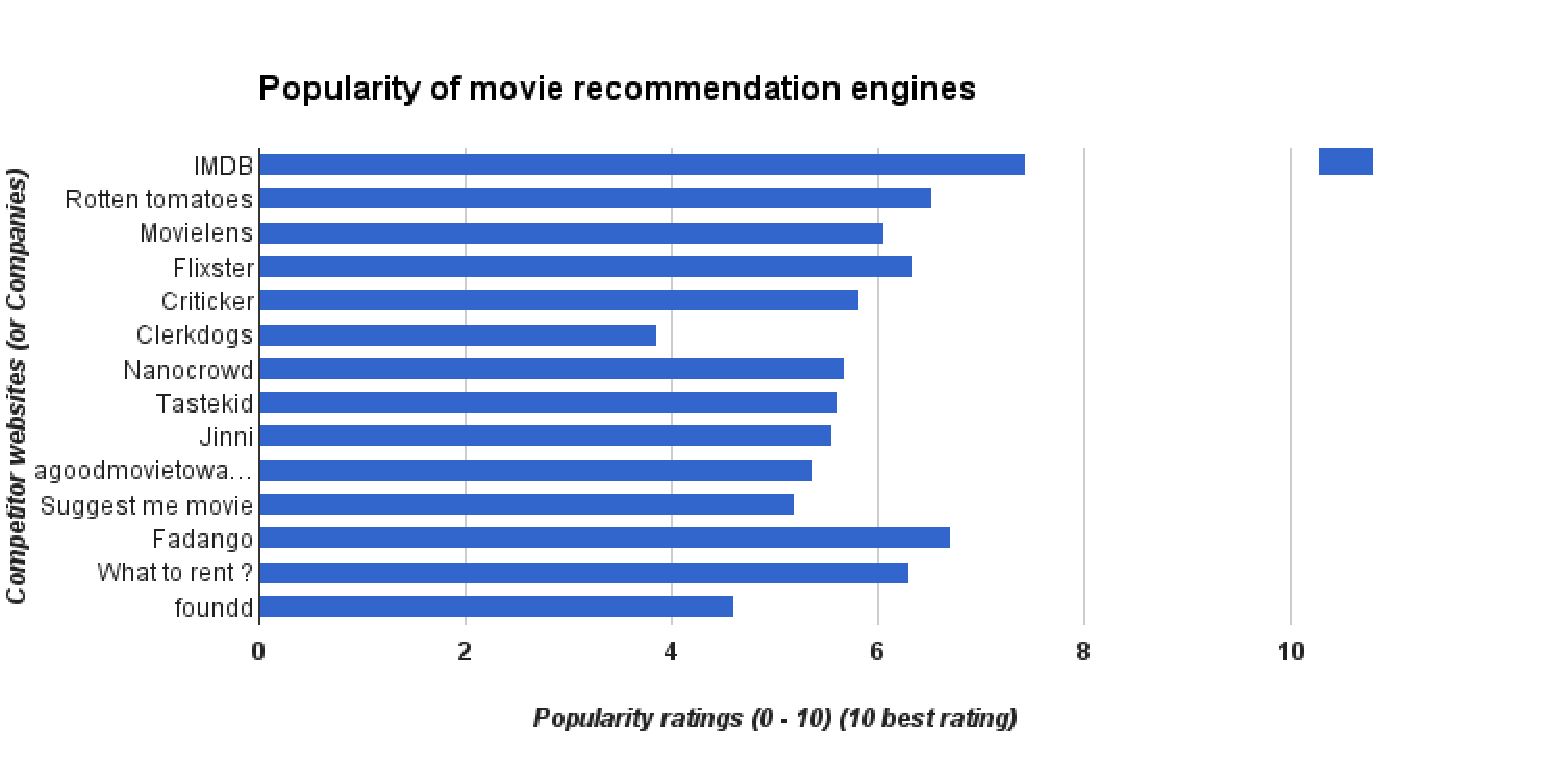
\includegraphics[scale=0.7]{Figures/competitor_popularity.pdf}
		%\rule{35em}{0.5pt}
	\caption[Graph: Popularity rating of competitors in the area of movie recommendation system]{Popularity of Vionel's competitors \citep{popularity_online}}
	\label{fig: Popularity of competitors}
 \end{figure}

 \begin{figure}[htbp]
	\centering
		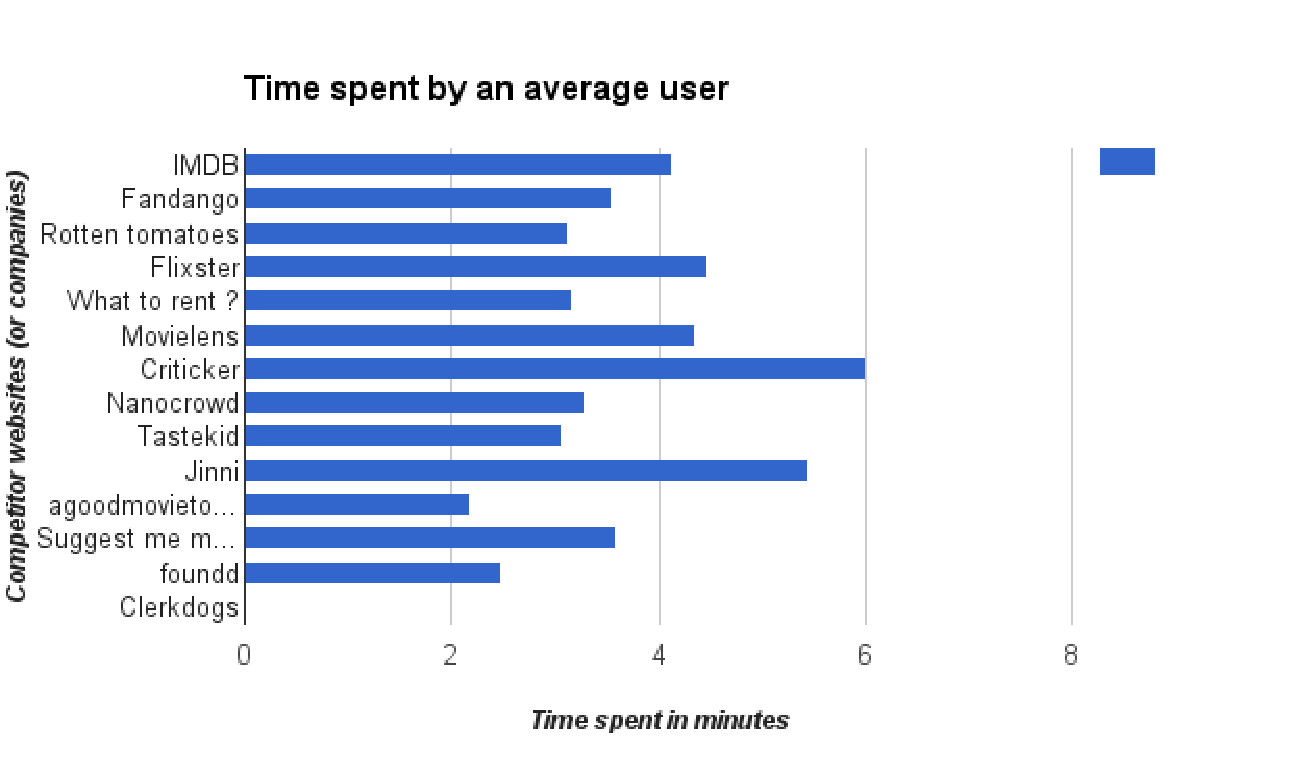
\includegraphics[scale=0.7]{Figures/fig_time_spent_each_recommender_site.pdf}
		%\rule{35em}{0.5pt}
	\caption[Graph: Average time spent by an user in popular movie recommendation websites]{Time spent by an average user in recommender websites\citep{Alexa_imdb}}
	\label{fig: Time Spent by an average user}
 \end{figure}

  
\section{Competitive advantage and technological differentiation}
\label{Competitive_advantage_tech_differentiation}
 For any company to beat the competitor to the market, there is a need for company to out think and produce a product that provides better value for customers at relatively same or less price. Technological development in a company's product which helps outranking competition in any form is essential to mark the presence of a firm in industry by gaining competitive advantage. In the domain of movie recommendation systems, technology plays an vital role in determining value provided to the customer and also helps in differentiating a product from its competitors. As described by Micheal Porter in \citep{Porter199806}, technological developments not only boosts the metric of differentiation from its competitors but it also increases firm's competitive advantage by influencing uniqueness of a product. Hence there is need for investments in research and development to improve recommendation algorithm. 

 Sustainable competitive advantage is achieved when a product of the company is able to provide a better value to the customer and continues to do so for a longer duration of time by creating barrier for other competitors to persuade its customers to switch the product. In the case of technology driven startups, sustainability is most of the times achieved by developing an highly innovative product or solution to the customers. As described by Byers and Nelson in \citep{ByersDorfNelson201401}, One more strategy of achieving sustainability is by collaborating with suppliers, complementers and other companies, which help in creating ample opportunities for development by building an sustained business ecosystem . The aim of collaborative strategies is to create powerful barriers for new entrants to enter into market segment. More about how Vion Labs is changing its strategy to achieve sustainable competitive advantage is described in section \ref{Changes_needed_to_face_the_challenge} of the report.  

\section{Information about Vionel's competitors}
 Since research question is about comparing features provided by \acrshort{MRS} in current market, five competitors are chosen to perform analysis and compare with Vionel. The following subsections provide overview of chosen competitors in the areas of unique features provided by them, revenue model used by them, the companies they have tied partnership with and also information about customer's view regarding recommendations offered. A critical aspect to study about competitors is to understand problems faced by them and the strategy used to overcome it. The following subsections capture all the related required information. Knowledge of unique features provided by competitors, helps us to rethink features provided by Vionel and improve our service. Inclusion of some features requires partnerships with other companies, hence partnership information of each competitor is collected during competitor survey. If some competitors use advertisement based revenue model, the web outlook feature of recommender system is greatly affected also, revenue model of competitors will help us to understand the underlying features in the framework. Finally, customers viewpoint about the service offered is summarized to compare it with Vionel and understand expectations of end users.     

 \subsection{Internet Movie Database Inc. (IMDB)}
  \label{IMDB_overview} 
  \subsubsection{Differentiating features}
    \label{IMDB_overview_DF}
    \acrshort{IMDB} has a wide collection of movies from all over the world, in fact it has highest collection of movie titles, related data items under one domain name. \acrshort{IMDB} supports both content based and collaborative based filtering to power its recommendation engine. Content based recommendations are as good as available content, \acrshort{IMDB} has around 180 million data items related to movies \citep{Press_imdb_online}. Currently the personalized recommendations are produced by collecting user's choices by monitoring on movies bookmarked by a user. Recommendations are not limited to popular movies, algorithm suggests movies from the non-popular category too. Recommendations are based on similar genre, tempo of the movie, similar actor and plot. It also cover movies from other languages, which have similarity to user's taste. One distinguishing feature is that it explains the reasons for suggesting a movie to the user, this creates a sense of assurance about quality of recommendations. \acrshort{IMDB} website outlook is easy to navigate, external advertisement free, provides information about new releases, suggestive movie lists from other users, actor and character information. It provides provision for users to navigate and search through movie content based on certain movie tags, for instance ``Movies based on Novels''.  

    \acrshort{IMDB} ratings are assigned to each movie content, based on its popularity among the users. A five star based rating information collection method from users is adopted to generate average ratings for a movie. Users are encouraged to cast votes for data items, including movie actors and movies.    
  \subsubsection{Revenue model}
    \label{IMDB_overview_RM}
    \acrshort{IMDB} uses cost per action (CPA) based revenue model in its website, the actions here refer to a user buying a movie using links provided in the website. With the recent acquisition of it by well know on-line retailer Amazon, it is clear that the trend is moving in the direction where retailers are buying out related publishing websites like \acrshort{IMDB} to improve their sales of movie DVDs, other movie related goodies \citep{How_I4_online}. Hence the core algorithm of \acrshort{IMDB} has modified to boost the sales of movie content providers like Amazon, also there is inclusion of ``buy from'' feature in website. Hence it can be observed that there is influence of revenue model to some of the features of a movie recommendation website. 
  \subsubsection{Information about partners}
    \label{IMDB_overview_IP}
    Partnerships with movie information content providers defines the quality of movie information that will be used for recommendations. Hence partnering with renowned movie production houses is essential for a company which has movie recommendation engine as product. \acrshort{IMDB} has partnerships with a good amount of movie production houses including other language movie production houses. Also partnership with on-line retailers and on-line movie on demand services is crucial for attracting more number of users. Some of the partners of \acrshort{IMDB} are MFP Munich Film Partners GmbH \& Company, Silver screen partners, Merced media partners, Armada partners, DirecTV and many more.   
  \subsubsection{Shortcomings and problems in recommendation algorithm }
    \label{IMDB_overview_SP}
    \acrshort{IMDB} requires the users to bookmark and rate at least twenty movies to be able to generate personalized movie recommendations. Most of the users tend not to bookmark and rate the movies that they like by searching for them manually. The quality of recommendations generated is as good as its input, hence \acrshort{IMDB} suffers from a cold start problem for each user. Currently, the recommendations are based on movie features like genre, popularity, actor similarity and character similarity, but there is room for including other features of movies to predict similarity between them for better prediction. 
     
  \subsection{Fandango Inc}
   \label{Fandango_overview}
   \subsubsection{Differentiating features}
   Fandango provides it users with a comprehensive search engine to find movies they like and also provides links to buy tickets if the movie is played in nearby cinema theaters. The search of movie theaters uses location information of the users. Movie reviews presented to users comprise of both critic based and registered user based reviews. Recommendation system uses both film critics based ratings and user based rating values for recommending movies to users. One innovative feature for benefit of parents is added, which alerts the users about allowed age for viewing a particular movie content. The five pointer rating meter is linked with abusive language, violence, scary scenes and other age restricted content for each movie. It also allows movie content such as posters, trailers, plot synopsis to be published in the website. Recommendations are content based, it uses movie genre, plot, actors and related data items to suggest movies to the user. A feature of allowing users to create alerts for a movie and get notified if there are movie tickets available in local theaters. 
  \subsubsection{Revenue model}
  \label{Fandango_overview_DF}
   Fandango has revenue model based on sales of movie tickets online. The recommendation engine suggests a newly released movie ,along with the link to buy tickets to watch movie in movie theaters. Unlike \acrshort{IMDB}, it has coupled a website publishing a movie content to movie theater franchises where movies can be watched in nearby locations to the user.    
  \subsubsection{Partners information}
  \label{Fandango_overview_IP}
   Fandango has partnered with Samsung TV to publish movie information in the form of trailers and also location based personalized links for users to buy movie ticket \citep{Fanda7_online}. The main partners for Fandango are movie theaters, some of the noticeable partners are AMC theaters, Premiere theaters, Georgia theater companies and many more.
  \subsubsection{Shortcomings and problems in recommendation algorithm } 
  \label{Fandango_overview_SP}
   The general image of Fandango among customers is that it is a website which sells movie tickets. Less number of people use it as a discovery platform to search for older or not so popular movies. Recommendation engine is biased towards movies that have tickets availability in theaters nearby to location of users.     

 \subsection{Jinni Inc}
  \label{Jinni_overview}
  \subsubsection{Differentiating features}
   Jinni provides its user with a personalized movie recommendations based on their entertainment personality, mood and taste. Unlike \acrshort{IMDB}, Jinni asks its users to chose short phrase related to type of movie to watch, such as ``Movies with scary storyline''. It contains around 40 -60 reliable tags for each movie title. It allows users to import ratings from other movie recommender websites, by reliving the pain of users to search for movies they like and re-rate them. Once the recommendation learns more about the user's taste, the recommendations generated are highly accurate and surprising. One more feature that is interesting for the users is to allow them to filter movies based on place, for instance if a user selects ``England'', all the movies related to this keyword are displayed to the users along with its trailers. Likewise, Jinni is planning to include speech based searches to enhance user engagement in website and on smart TVs \citep{Jinni0_online}. These features enable easy navigation for users with little or no computer knowledge. In the area of innovativeness, Jinni is found to be the best among the competitors.   
  \subsubsection{Revenue model}
  \label{Jinni_overview_RM}
    Jinni is in the path of creating an entertainment genome, which enables the algorithm to recognize a person's personality based on movies liked. The historical information about users watched content is used by Jinni to provided better entertainment recommendations for user in future. It provides services for smartTV and other over-the top content providers to provide personalized recommendations for users based on collected user data. For websites that host advertisements in the form of videos, Jinni provides application programming interfaces for generating personalized recommendations for its users.    
  \subsubsection{Partners information}
  \label{Jinni_overview_IP}
    Jinni recommendation api's are capable of predicting user behavior by using historical data collected. Any web related infrastructure where users are allowed to view videos, the api's are capable of generating personalized recommendations, hence some of the mobile application developing companies, web applications developers, smartTV providers, set up box providers have become partners with Jinni. The partners are Arris, seaChange, NDS and openTV. Hence Jinni's recommendation algorithm makes use of collected user data over a period of time to suggest movies in future with high accuracy. 
  \subsubsection{Shortcomings and problems in recommendation algorithm }
  \label{Jinni_overview_SP}
    Jinni's recommendation engine faces the problem of cold start for new user, for which algorithm has no history of collected data with it. Currently to solve the problem, soon after registration user needs to rate movies based on their tastes to enable algorithm to generate recommendations based on that list of movies. If a user is unwilling to do that there is a problem of user getting frustrated and leaving the service. 

  \subsection{A good movie to watch }
  \label{agoodmovietowatch_overview}
  \subsubsection{Differentiating features}
  \label{agoodmovietowatch_overview_DF}
    A good movie to watch provides its users with an on-line platform to discover popular movies based on their taste, also there is provision for discovering movies which are less known among the public. The website has a simple structure comprising of options for users to select tags for a movie to watch. The recommendations are content and ratings based, there is a high possibility that movies with less box office splash to come up in the list of recommended movies for the users. One of the interesting feature of this website is that it allows users to search for movies to be watched with a group of friends, family, crush or also movies to be watched alone. The innovativeness in the features provided by this website is good. It has links where to watch the liked movie content from, most of the times it is pointing to Netflix.
  \subsubsection{Shortcomings and problems in recommendation algorithm }
  \label{agoodmovietowatch_overview_SP}  
    The major shortcoming in this website is that the movie content starts from year 1982, it is a niche dataset with good quality movies in it.
    Database is built upon movies that have more than 6.7 movie ratings in \acrshort{IMDB} and more than 60 percent score in Rotten tomatoes \citep{Agoodmovietowatch_online}. Website lacks movie trailers that are essential for engaging movie enthusiasts to stay for more duration in  website.  

  \subsection{Foundd Inc}
  \label{Foundd_overview}   
  \subsubsection{Differentiating features}
  \label{Foundd_overview_DF}
    Foundd provides its user with a personalized recommendations based on their tastes and has a feature of collaborating with friends in social media websites. Provides a better user friendly, advertisement free web interface to browse through movie and TV series content. Mood based movie filtering is also a part of Foundd's content discovery platform. Users have to provide information about their entertainment personality to the recommender engine to start receiving movie suggestions. All activities on Foundd website are made socially available to friends in social media platforms. User privacy settings are allowed to change, there is provision for sharing rated movies history information with other users on Foundd. It has a continuously updated blog in web page to engage users to provide comments about overall service provided to them. It has feature of providing information about where to watch a movie, Netflix and other movie on demand website links are provided along with the displayed movie information.     
  \subsubsection{Shortcomings and problems in recommendation algorithm}
  \label{Foundd_overview_SP}
    Foundd also faces the problem of cold start that forces its users to manually search and rate at least ten movies they like in order to obtain good recommendations. Ratings based on film critics is missing, the ratings are only based on views of users on Foundd. Provision of filtering movies based on mood of a user is lacking. There is chances of creating an unreliable movie recommendation system, if the users are creating fallacy ratings for movies by deliberately trying to spoil rating system. Hence ratings from film critics also needs to be used to solve the problem of corrupt ratings. 
    
 
% Chapter 3
\chapter{Achieving sustainable competitive advantage} % Main chapter title
\label{Chapter3} % For referencing the chapter elsewhere, use \ref{Chapter1} 

\lhead{Chapter 3. \emph{Achieving sustainable competitive advantage}} % This is for the header on each page - perhaps a shortened title

\setstretch{1}
%----------------------------------------------------------------------------------------

\section{Comparative analysis}
  % About Jinni's growth due to technological differentiation ... explain 
  In previous section, information about features used by companies to provide movie recommendations to users are summarized. Since the goal of this report is to compare features provided by our competitors and to understand how technological differentiation in developed product increases the possibility of achieving sustainable competitive advantage. Popularity index of a movie recommendation engine in current situation is as shown in figure \ref{fig: Popularity of competitors} , a websites popularity entirely depends on the number of unique visitors making use of the recommendation service. It becomes crucial to understand the reasons behind popularity of a particular website, this information helps in contrasting it with its competitors to know more about their success strategy in both technical and business domain. 

  On the technical front, features related to the core product, in our case movie recommendation engines are compared by using datum obtained during literature survey. A interesting metric for a website to be more intriguing to the user is time spent by an average user in viewing the content, the graph in figure \ref{fig: Time Spent by an average user} displays this information. A noticeable observation in this graph is about time spent by an average user in Jinni website, despite of it being a new company compared to \acrshort{IMDB} there is a high viewing time by visitors. The reason is that Jinni has innovative features not limited to mood based recommendations, user friendly interface and easy import of rating data from other recommendation websites. More about features that are essential for a recommender website to gain popularity are compared in following subsection \ref{Comparision_of_features} and comparing Vionel's planned features with features provided by state of the art recommender engine in current market in subsection \ref{Comparision_with_state_of_the_art}.        

 \subsection{Comparison of features}  
 \label{Comparision_of_features}
  
   \begin{figure}[htbp]
	\centering
		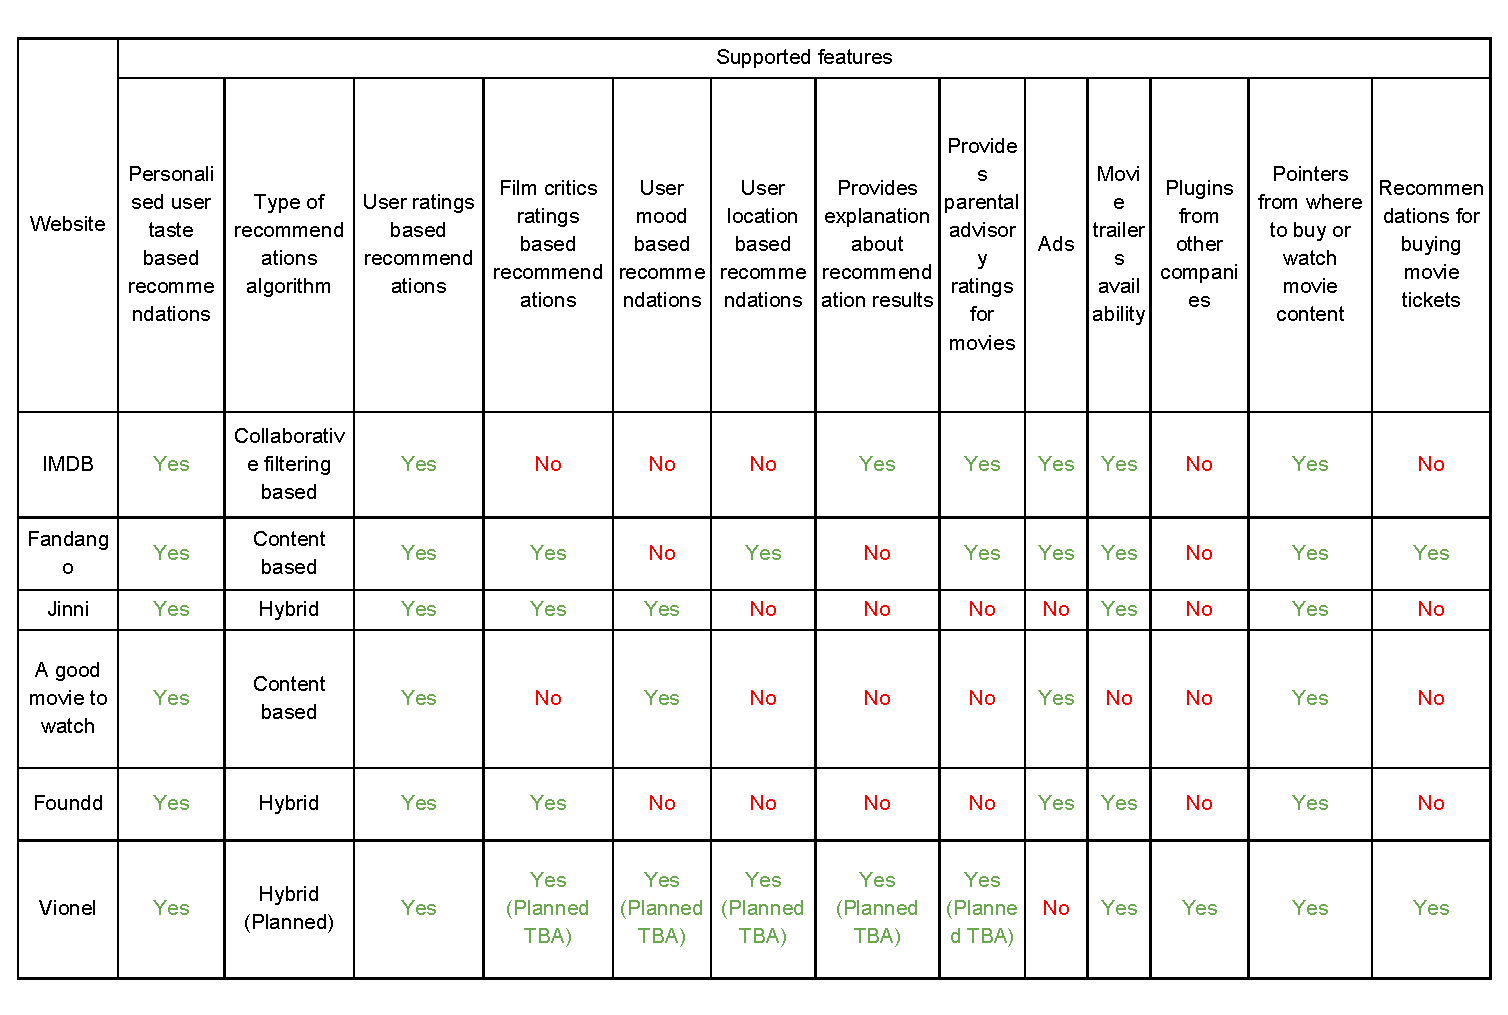
\includegraphics[scale=0.6]{Figures/Features_comparison.pdf}
		%\rule{35em}{0.5pt}
	\caption[Table : Summarized feature comparison table]{ Summarized feature comparison table}
	\label{Table: Feature comparison}
   \end{figure}
    
   As shown in the table \ref{Table: Feature comparison}, the distinctive features of movie recommendation engines are tabulated in order to enable faster comparison of features provided by each website. By comparing features provided along with the information of popularity of websites, provides clue for which feature is crucial for a website to be popular among users. Our fierce competitor \acrshort{IMDB} has a large fan base, the reason for its popularity is sheer amount of movie information it contents. In spite of attracting more number of users, \acrshort{IMDB} is unsuccessful to engage users for longer duration in website. Whereas, a recent innovative startup from Israel, Jinni is able to retain users for longer duration of time. The reason for Jinni to be so engaging is provision for users to search for movies in an innovative way based on mood information and also based on other innovative tag category for movies. Most of the older recommendation engines either use content based or collaborative filtering based recommendation algorithms. The algorithm should use both user ratings and film critics ratings for generating recommendations. Websites that only use user's rating based recommendations have a danger of suggesting irrelevant movies to the user, if the collected rating information for a movie is corrupted deliberately by users. Hence, Vionel is planning to use both user ratings and film critic ratings to generate recommendations. New startups such as Foundd, Jinni have a combination of both content based and collaborative filtering based algorithms to better match taste of the user. An innovative feature of providing information about the type of content in the movie is part of \acrshort{IMDB} and Fandango's website, which is a better feature to have parental advisory control for display of movie content. A company Fandango provides content based recommendations, along with this it provides users with a suggestive list of links from where movie tickets can be purchased. This feature has made this website quite popular and it has become a goto location for all movie enthusiasts in USA. Vionel has already adopted its architecture to suggest users with the information of availability of movie content.  

   Advertisement free environment is appreciated by users of the website, on the other hand users enjoy availability of plug-ins from other companies containing songs from movies and trailers, in movie information catalogue. Hence it is planned to support these features which are popular among users to Vionel website, in order to attract more users. Also on top of this there is a need to innovate and add other features related to recommendations, more information about adding new technical features and how these features help in attaining competitive advantage are discussed in subsection \ref{Technical_changes_to_increase_uniqueness}.  

 \subsection{Comparison with state of the art}
 \label{Comparision_with_state_of_the_art}
 % compare and write the same thing , tech , biz etc
 The task of competitor analysis is to understand the factors that enabled a competitor to succeed, and use this knowledge to improve the condition of current product. In movie recommendations, \acrshort{IMDB} is undoubtedly the state of the art in terms of availability of movie content and also quality of recommendations provided. The backbone of recommendations is based on user's movie rating data, and \acrshort{IMDB} has collected this information from past decade to become a largest movie information database. In order to compete, Vionel has to collect more user data, and also movie information by creating ties with movie production franchises and companies that have user data related to entertainment. 

 Interesting and distinctive features from all of the competitors are used as guiding light to build our recommendation system. An example of this is \acrshort{IMDB} has a large database, but uses collaborative filtering for suggesting movies to the user. Whereas it is planned to use both content and collaborative filtering in providing suggestions for users in Vionel. The feature of providing mood based recommendations are obtained from Jinni and company named ``A good movie to watch''. Since people like to receive recommendations based on mood and to find a not so popular movie with great subject to watch. In order to out rank the state of the art competitor, few features of an ideal recommendation engine as described in \ref{State of the art movie recommendation engine}, are planned to be included in Vionel. The features related to computer vision and machine learning are used to improve the current state of the recommendation engines. 
 
\section{Challenges for attaining competitive edge}
 % Challenge explanation,  
  Vionel faces challenges on both technical and business front. The challenges faced by Vionel in technical side are concerned with improving accuracy of recommendations, inclusion of new features by researching in the domain of computer vision and machine learning. The challenge of solving the problem of cold start in the case of recommendation engines. One more important aspect is about privacy issues related to usage of users private information, hence a challenge for Vionel is to provide quality recommendations by respecting user's privacy levels. Overall, Vionel is facing the challenge of being unique by innovating and creating a technical differentiation from its competitors.

  On the business front there is need for partnering with companies, to enable addition of innovative features. Also there is a challenge in creating a barrier to new entrants in the domain of movie recommendation engines. The solution for solving technical and business related challenges are discussed in further sections.     

\section{Changes needed to face the challenge}
 \label{Changes_needed_to_face_the_challenge}
 % tech,block diagram explanation , biz
 For a technology based startup like Vionel, the best way of attaining competitive edge is by introducing innovative features into their products. In order to enhance customer experience and increase the number of visitors, Vionel's \acrshort{MRS} should make use of innovative movie data analysis techniques to improve quality of recommendations provided to the user. To face the challenge changes has to be made in both technical and business front. Inclusion of few innovative features requires few business oriented changes such as partnering with complementers, suppliers and other companies that provide required data. The following subsections \ref{Buisness_related_changes} and \ref{Technical_changes_to_increase_uniqueness} explains about the steps that have been either initiated or planned to be incorporated in near future by marketing and R\&D team of the company respectively. The information about planned activity is collected from discussion with respective members of the team. All the changes are planned by objective of enhancing user's experience and to encourage more number of users to use Vionel's recommendation engines.

 % Spotify 
 \subsection {Business related changes} 
  \label{Buisness_related_changes} 
    Movie recommendations are as good as the database of movie information available at recommender algorithm's disposal. In order to improve the quality of recommendations, it is essential to add information about movies from all over the world. Currently, it has been planned to use open source movie databases to facilitate recommendations. Even though a complementer to our product such as Warner Bros., a movie production company, has ties with Vionel. To avail even more reliable movie meta-data, there is a need for building strong ties with other popular movie production agencies such as 20th century fox, Castle rocks entertainment, Marvel studios and many other complementors. By doing this there is high possibility of increasing the market share, as happened in the case of our fierce competitor IMBD Inc as mentioned in \ref{IMDB_overview_DF}.     
 
    All the content based recommendation engines face problem of cold start, it is a situation where recommender algorithm is clueless about a user's taste to suggest movies, especially in the case of newly joined users. In order to improve user taste based personalized recommendations, user's data has to collected from company which has access to it. There has been proposal to partner up with a popular telecommunication provider in Sweden to facilitate access to user's entertainment genome information. In exchange to this telecommunication provider uses Vionel's recommender algorithms to provide personalized entertainment recommendations to its users. The vision of creating a business ecosystem in the domain of entertainment recommendations is as described in figure \ref{fig: Proposed business ecosystem}. It enables Vionel to create a barrier for new entrants into Sweden's entertainment recommendation market. Additional feature of obtaining user data from other companies, allows new users who are part of any of the partnering companies to enjoy movie recommendations provided by Vionel right after registering in website.

    \begin{figure}[htbp]
	\centering
		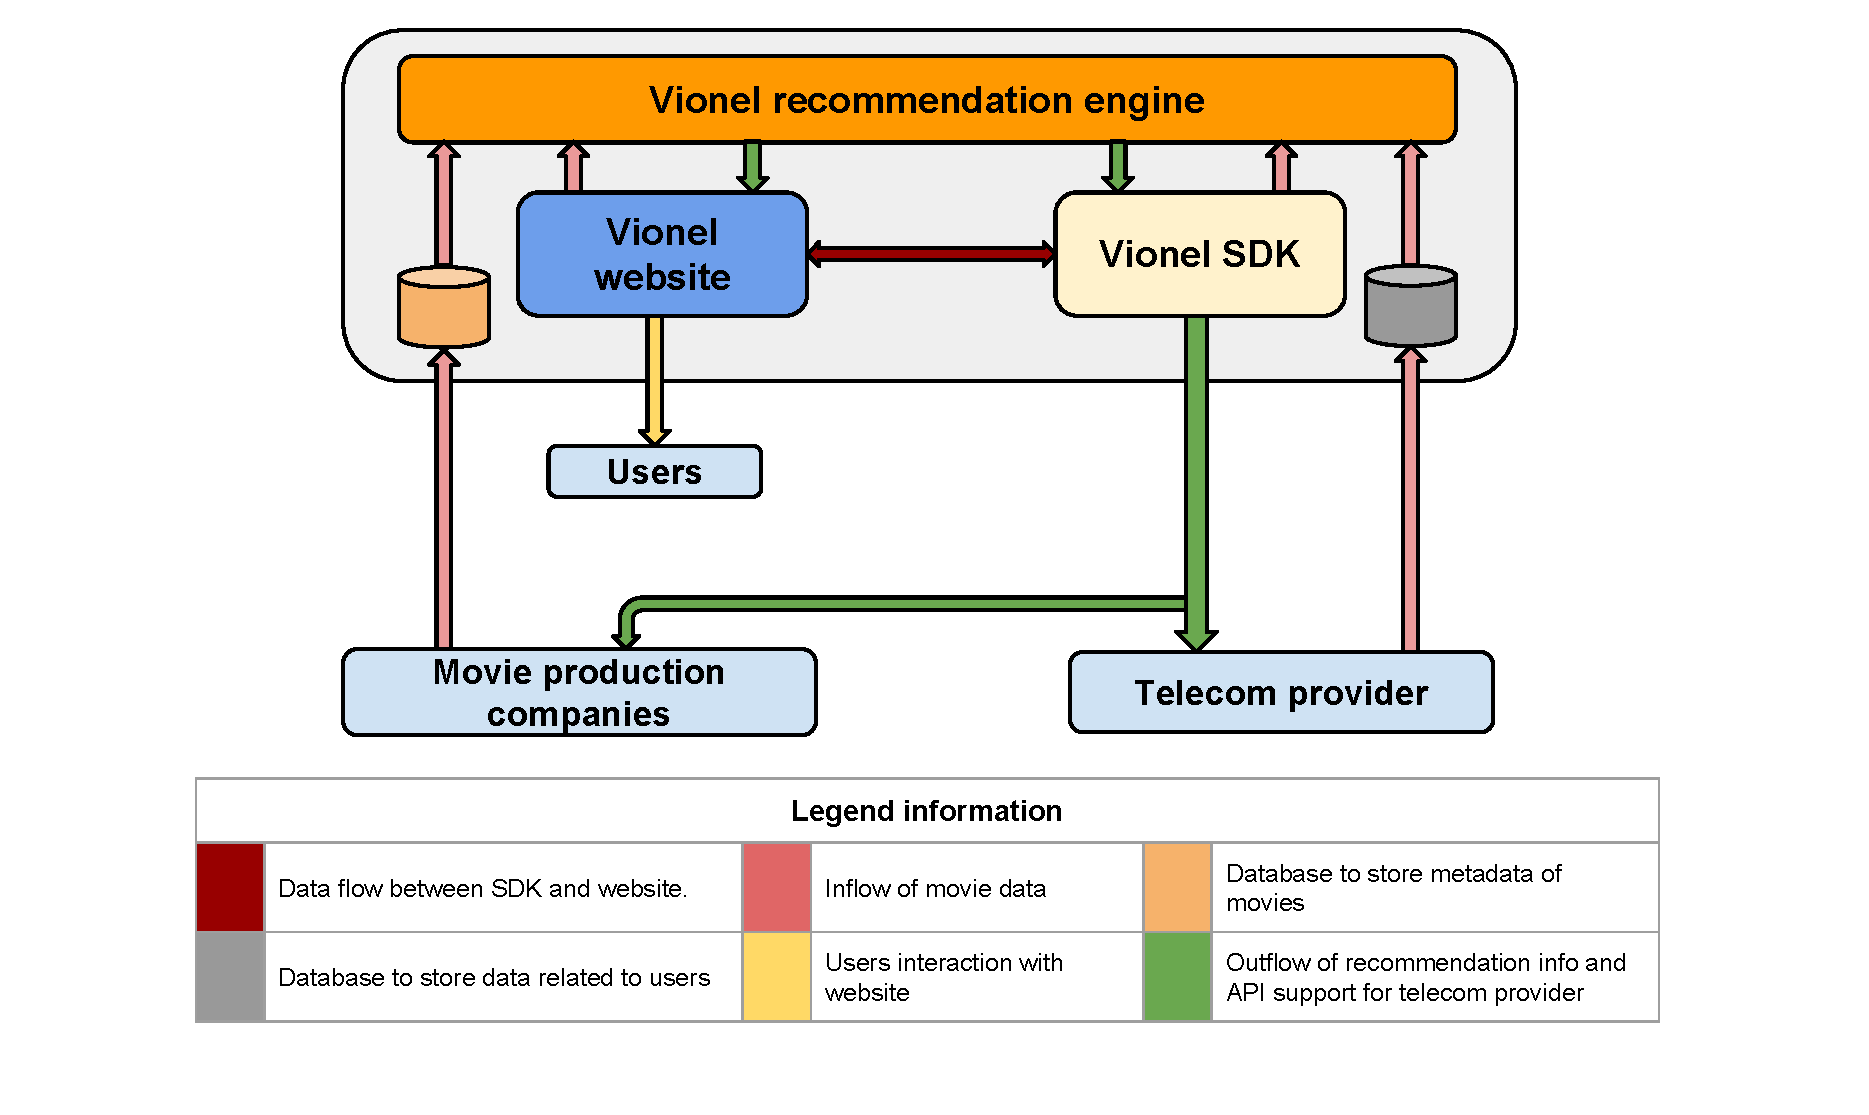
\includegraphics[scale=0.5]{Figures/Business_ecosystem.pdf}
		%\rule{35em}{0.5pt}
	\caption[Figure: Proposed business ecosystem]{Proposed business ecosystem, Source: Vion Labs marketing team}
	\label{fig: Proposed business ecosystem}
    \end{figure}  

 \subsection {Technical changes to increase uniqueness} 
  \label{Technical_changes_to_increase_uniqueness}
   % Spotify ,social media, innovative ratings (questionarie based), computer vision algos, hybrid recommender system. Where to watch ? , Mood based, voice based mood detection and movie suggestion, location based, time and day based, weather and mood based recommendations, surprises, mention about Jinni, how it used innovative solutions to gain competitive edge ...    
    As described in section \ref{Competitive_advantage_tech_differentiation} of literature study, the way of creating an good image in the minds of customers is by providing them with better valued product. In order to do so, there are changes required in the technical features of Vionel. The motto of web recommendation engines is to engage users by providing quality content and recommendations. To create technological differentiation of recommendations, several innovative ideas needs to be incorporated into architecture of recommendation systems. One such feature is to provide recommendations for a new user by solving the problem of cold start as described in section \ref{Buisness_related_changes} by developing Vionel software development kit to support inclusion of user's data as input to recommendation engine. The trend of recommendation engines is moving towards hybrid recommendation engines, where recommendations generated are combination of both content information and history data of user ratings. Vionel can benefit by adopting its technical architecture to support hybrid recommendations to its users. 

    Partnering with companies such as Spotify to get access to its customer data, in return providing space in website to publish songs related to movies. The quality of recommendations provided by Vionel can be further improved by getting access to songs liked by a user. Since, it is highly likely that a user liking a song from a movie, would like that movie or related movies. Overall, by using efficient user data analytics, a person's complete entertainment taste can be predicted accurately. On the other hand there is a possibility of getting access to user's personal data such as location, likes and dislikes info about a subject by respecting privacy of users, while partnering with social media companies. An ideal recommendation engine should provide suggestions to the user by recognizing user's mood at that instance, an effort in this lines has been considered by our competitor Jinni, which provides recommendations based on mood information selected by user. Other innovative features that could be used for the purpose of providing recommendations are based on user's location, time of the day, day of the week information and weather information, which influences mood of the users. 

    In a lateral dimension, computer vision algorithms combined with machine learning algorithms can be used to increase features that act as input to the recommender system. This involves movie content analysis to detect interesting features of movies like environment information, product placement information, color information, speed of the movie and others to generate large category of tags for movies. The feature of voice based navigation through website is an interesting feature to add, along with this a machine learning algorithm can be used to detect mood of a person based on voice information and it can be later used to recommend movies. A computer vision based method of detecting user's mood uses the technique of facial expression interpretation by capturing real time video feed. With this feature users who have little or no computer knowledge, especially elderly people will be able to use Vionel, with voice based navigation movie search feature. These innovative features will attract more number of users and also would encourage them to use our recommendation services before watching a movie.     

\section{Teams role in attaining competitive edge}
 % tech team , marketing team
 %R \& D team responsibility,  
    Achieving competitive sustainable advantage is a collective effort from all member teams of a company. The respective responsibilities that needs to taken by the teams are as follows:
    \begin{itemize}

    \item CEO and Marketing team members : 
    The role of marketing members is to find partners ranging from movie production franchises, movie content providers and companies that are willing to embed plug-ins (example: Spotify). In order to improve discovery of the website, actively participating in press related events, representing organization in business events, startup meets to attract investors. Finally, to create a sustainable business ecosystem where Vionel can thrive upon by inhibiting other competitors in the business and creating a powerful barrier for new entrants in movie recommendation business.  
    
    \item Research team members : 
    The main responsibility of adding innovative features by performing research to enhance the capabilities of recommendation engines is with research team members. Adopting high tech methods of research to develop and improve recommendation algorithm that supports multiple type of recommendations. Development of baseline recommender engine on top of baseline movie content discovery framework.
    
    \item Development and production unit team members : 
    Development team members ensure faster development of researched features and publish it in the website. Other responsibilities of team members involve ensuring faster response time, avoiding website downtime, developing user friendly web pages for the website, efficient handling of user data, and recommendation SDK development. 

    \item Personal relationship (PR) team members : 
    PR team members responsibility is to collect opinions from the users, answer queries related to website content, and also to receive customer complaints, suggestions regarding Vionel product. This information has to passed over to research team to facilitate addition of new feature into recommendation system.

    \end{itemize}  
       
\section{Contribution from internship work}
 % innovative feature for recommender systems
   The main contribution from the internship work is to enable automatic brand logo detections in movies. The process of detecting brand logos in movies is tough job for humans, hence internship effort was to perform the task of brand logo detection using computer vision algorithm combined with machine learning technique. One more important contribution was to reduce the time taken for extracting features from movies using cluster of graphical processing units. Currently brand logo detector can detect ten specific brands from movies to create tags for recommendation engine to improve its suggestions to users. A framework is created to include brand logos of other companies in future, to generate accurate tags from movies. There has been considerable reduction of processing time per movie by using computational power of GPUs. Currently the time taken for processing and generating tags has been halved with the use of two GPUs in parallel. Future projects can use the developed framework to parallelize extraction of features using machine learning techniques on videos. These contributions help R\&D team to innovate more by faster prototyping of ideas, it can also be used to generate more tags automatically from new movies that are added into the database. Reduction in time and addition of innovative tags increases technical differentiation from our competitors, thereby helping Vionel to achieve competitive edge in view of customers.        

\section{Conclusion}
 % How technological differentiation enables a company to attain competitive edge over other companies. Write about next step in innovation processes
   Comparative analysis of features supported by companies has increased knowledge about competition, also information about driving factors that enables a movie recommendation product to be popular have been critically accessed. Gained knowledge during the analysis could be used during next stage in the innovation process for \acrshort{MRS} product. Especially, the collected information helps in early identification, during ideation phase, the critical features that should be supported by Vionel to achieve success. A clear understanding of how technical differentiation of a product assists a company to achieve sustainable competitive advantage is characterized in the case of movie recommendation industry. Overall, this report takes one step further in innovation framework for recommendation engine product of Vion Labs. It provides valuable information of highly competitive companies in the market, which can be further used to determine competitive strategies to achieve sustainable competitive advantage by attracting and retaining more number of users.
%\input{Chapters/Chapter4} 
%\input{Chapters/Chapter5} 
%\input{Chapters/Chapter6} 
%\input{Chapters/Chapter7} 

%----------------------------------------------------------------------------------------
%	THESIS CONTENT - APPENDICES
%----------------------------------------------------------------------------------------

%\addtocontents{toc}{\vspace{2em}} % Add a gap in the Contents, for aesthetics

%\appendix % Cue to tell LaTeX that the following 'chapters' are Appendices

% Include the appendices of the thesis as separate files from the Appendices folder
% Uncomment the lines as you write the Appendices

%% Appendix A

\chapter{Appendix Title Here} % Main appendix title

\label{AppendixA} % For referencing this appendix elsewhere, use \ref{AppendixA}

\lhead{Appendix A. \emph{Appendix Title Here}} % This is for the header on each page - perhaps a shortened title

Write your Appendix content here.
%\input{Appendices/AppendixB}
%\input{Appendices/AppendixC}

%\addtocontents{toc}{\vspace{2em}} % Add a gap in the Contents, for aesthetics

\backmatter

%----------------------------------------------------------------------------------------
%	BIBLIOGRAPHY
%----------------------------------------------------------------------------------------

\label{Bibliography}

\lhead{\emph{Bibliography}} % Change the page header to say "Bibliography"

\bibliographystyle{unsrtnat} % Use the "unsrtnat" BibTeX style for formatting the Bibliography

\bibliography{Bibliography} % The references (bibliography) information are stored in the file named "Bibliography.bib"

\end{document}  
